\section{Additional Results for \qwen}
\label{app:qwen}

\Tabref{tab:qwen_baselines} gives the per-task baselines for \qwen, and \tabref{tab:qwen_interference} the pair matrix.
\Figref{fig:qwen_retention}, \figref{fig:qwen_h1}, and \figref{fig:qwen_h3} repeat the main figures for \qwen.

\begin{table}[h]
    \centering
    \small
    \begin{tabular}{@{}lcccc@{}}
        \toprule
        \textbf{Task} & \textbf{Zero-shot} & \textbf{End of own stage} & \textbf{Sequential, end of run} & \textbf{Joint multi-task} \\
        \midrule
        \tgsm & {\bf 0.475} & 0.461 & 0.376 {\scriptsize (0.153)} & 0.430 \\
        \tarith & {\bf 0.985} & 0.981 & 0.839 {\scriptsize (0.195)} & 0.975 \\
        \tlogic & 0.595 & {\bf 0.712} & 0.622 {\scriptsize (0.108)} & 0.680 \\
        \tmt & {\bf 0.469} & 0.465 & 0.436 {\scriptsize (0.035)} & 0.466 \\
        \tsumm & 0.269 & {\bf 0.338} & 0.309 {\scriptsize (0.012)} & 0.324 \\
        \temo & 0.500 & {\bf 0.910} & 0.817 {\scriptsize (0.108)} & 0.855 \\
        \midrule
        Mean & 0.549 & {\bf 0.644} & 0.567 & 0.622 \\
        \bottomrule
    \end{tabular}
    \caption{Per-task metrics on \qwen (6 sequential runs; joint training 1 seed; standard deviation over runs in parentheses). Best value per row in {\bf bold}. Fine-tuning does not improve \tgsm, \tarith, or \tmt.}
    \label{tab:qwen_baselines}
\end{table}

\begin{table}[h]
    \centering
    \small
    \begin{tabular}{@{}lcccccc@{}}
        \toprule
        \textbf{Old $\backslash$ new} & \tgsm & \tarith & \tlogic & \tmt & \tsumm & \temo \\
        \midrule
        \tgsm & -- & 0.34 & 1.07 & 0.09 & $-0.06$ & $-0.12$ \\
        \tarith & $-0.70$ & -- & 1.46 & 0.01 & $-0.93$ & 0.53 \\
        \tlogic & $-0.07$ & 0.33 & -- & $-0.07$ & 0.10 & 0.19 \\
        \tmt & $-0.11$ & $-0.58$ & 1.13 & -- & $-3.56$ & $-1.78$ \\
        \tsumm & $-0.08$ & $-0.10$ & 0.30 & 0.06 & -- & 0.11 \\
        \temo & 0.02 & 0.05 & 0.06 & 0.03 & 0.06 & -- \\
        \bottomrule
    \end{tabular}
    \caption{Pair structure on \qwen: mean \rloss lost by an old task (row) during one stage of a new task (column). The \tlogic column is the largest in four of the five rows. The \tmt row is distorted by a near-zero denominator ($L_0 - L^* = 0.033$ nats).}
    \label{tab:qwen_interference}
\end{table}

\begin{figure}[h]
    \centering
    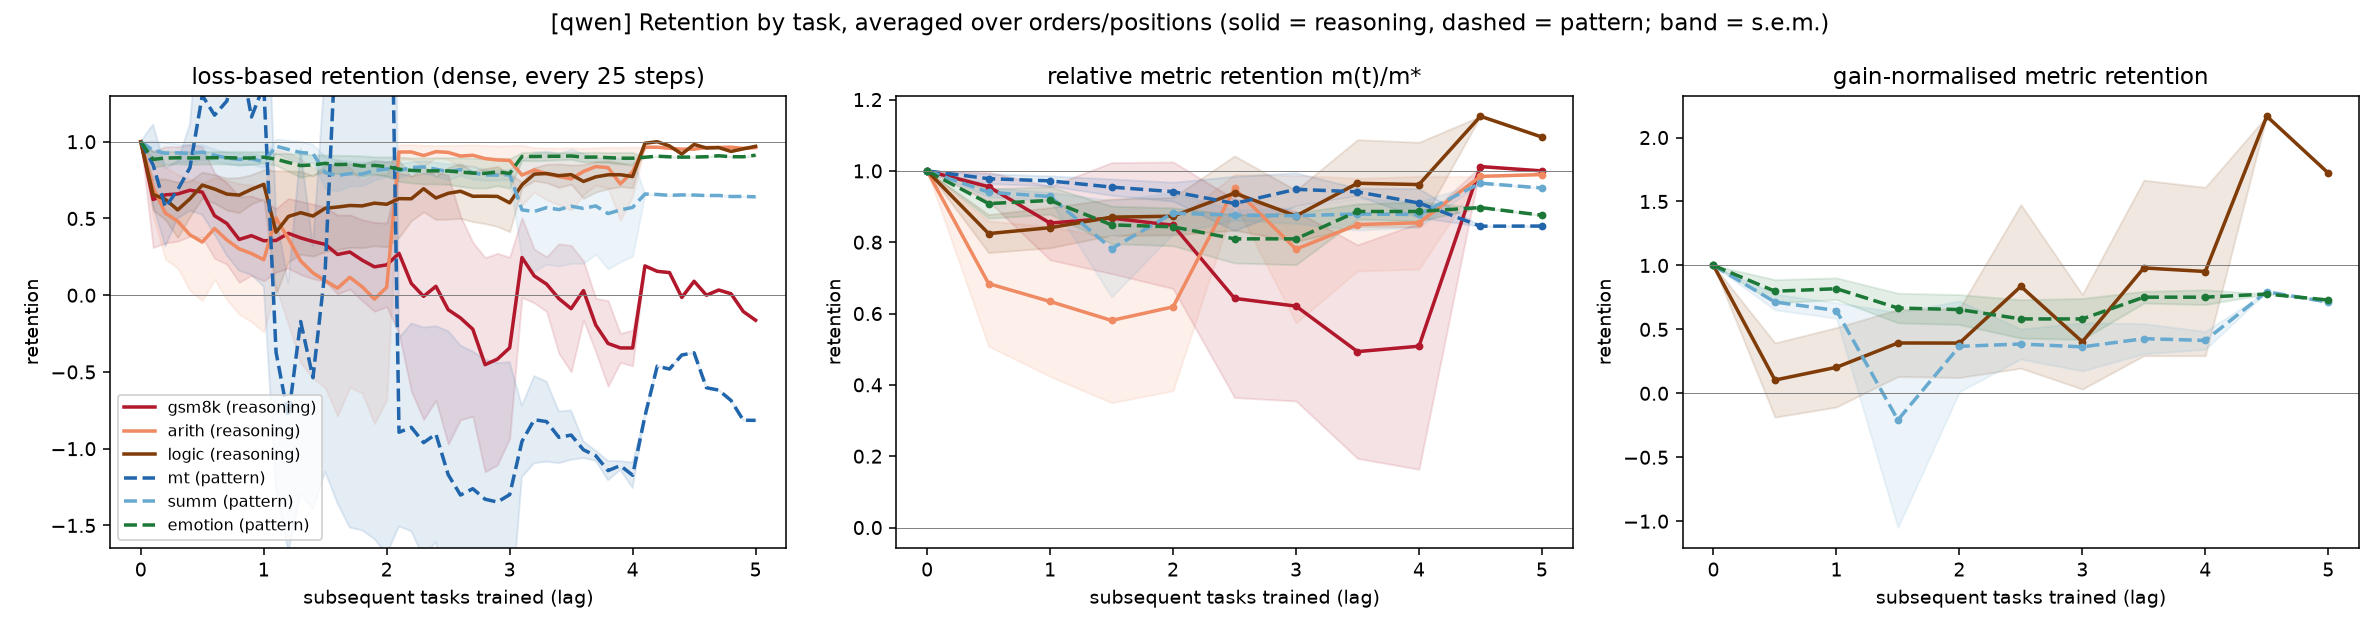
\includegraphics[width=\linewidth]{figures/qwen_retention_by_task.png}
    \caption{Retention by task on \qwen, averaged over orders and positions. Panels as in \figref{fig:retention}.}
    \label{fig:qwen_retention}
\end{figure}

\begin{figure}[h]
    \centering
    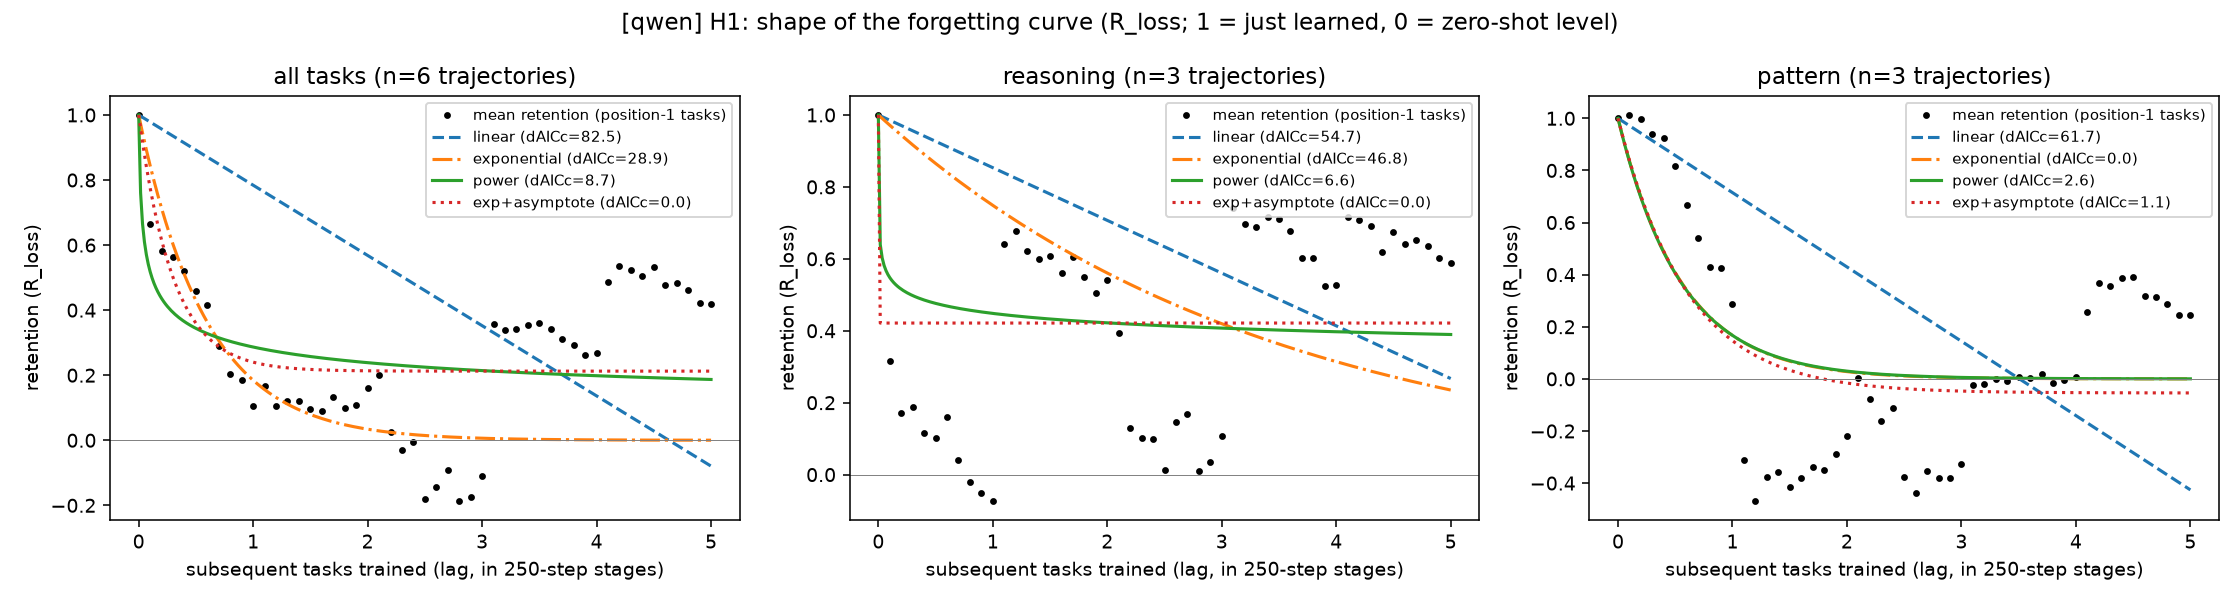
\includegraphics[width=\linewidth]{figures/qwen_h1_shape_R_loss.png}
    \caption{H1 fits to mean \rloss curves of position-1 tasks on \qwen. No smooth curve fits well (\tabref{tab:h1_mean}).}
    \label{fig:qwen_h1}
\end{figure}

\begin{figure}[h]
    \centering
    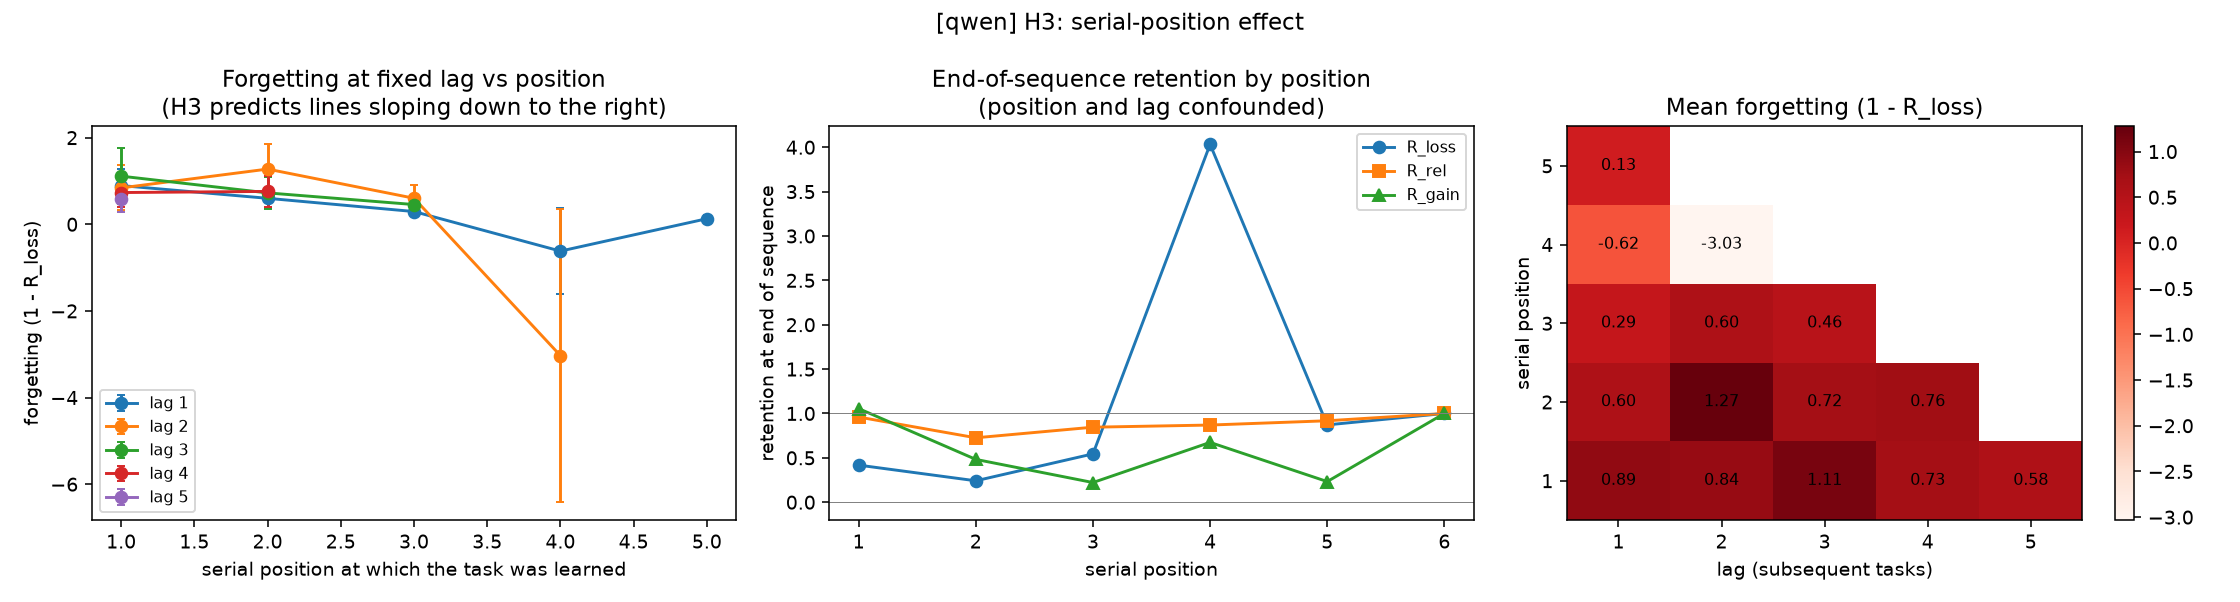
\includegraphics[width=\linewidth]{figures/qwen_h3_position.png}
    \caption{H3 on \qwen. Panels as in \figref{fig:h3}.}
    \label{fig:qwen_h3}
\end{figure}

\section{Sensitivity of the H2 Ratio on \llama}
\label{app:sensitivity}

We ran two exploratory sensitivity checks on the \llama category ratio.
By seed block, the unclipped \rloss ratio is 1.82 in block 0 and 1.15 in block 1; the clipped ratio is 1.06 and 0.95; the \rrel ratio is 1.23 and 1.07; and the \absdrop ratio is 1.43 and 1.24.
Leaving one task out, the unclipped \rloss ratio is 1.90 without \tgsm, 2.07 without \tarith, 0.43 without \tlogic, 3.52 without \tmt, 1.19 without \tsumm, and 1.08 without \temo.
The ratio therefore depends strongly on which single task is in or out of the comparison.

\section{Deviations from the Pre-registered Plan}
\label{app:deviations}

We wrote the analysis plan before any training run.
We deviated from it as follows.
\begin{itemize}[leftmargin=*,itemsep=0pt,topsep=0pt]
    \item \textbf{Evaluation cadence} (before any run). We planned loss and generation every 50 steps. We changed this to loss every 25 steps and generation every 125 steps, because generation costs about 45 seconds per evaluation point and loss about 3 seconds.
    \item \textbf{Generation budgets} (before any run). We raised the budgets for \tgsm and \tarith to 320 and 160 tokens, because a smoke test showed that verbose zero-shot answers were truncated before the final answer, which would have understated the zero-shot floor.
    \item \textbf{Full-fine-tuning ablation.} We cancelled it before any of its runs started. The GPUs were shared with other jobs, LoRA runs took up to about 100 minutes instead of about 10, and full fine-tuning needs about three times the memory. No full-fine-tuning data exists.
    \item \textbf{Restarts.} Two main runs and the \qwen joint baseline died with out-of-memory errors and were restarted from scratch with the same seed and configuration. We use no partial runs in any analysis.
    \item \textbf{Exploratory additions} (after seeing the main results). The clipped \rloss measure, the within-stage shape analysis, the equal-parameter per-trajectory comparison, the seed-block and leave-one-task-out sensitivity checks, and the onset experiment. A first attempt to get step resolution by re-running two full sequences with evaluation every 5 steps was aborted after 10 minutes because of its projected cost; we use no results from it.
\end{itemize}

\section{Compute and Software}
\label{app:compute}

We ran 18 sequential runs (12 on \llama, 6 on \qwen), 3 joint-training runs (2 on \llama, 1 on \qwen), and the six short onset runs on four shared NVIDIA RTX A6000 GPUs (48 GB), with a peak of 28 GB per process and bf16 autocast.
The full runs took 29.5 GPU-process-hours in total; because the GPUs were shared, single runs took 60--110 minutes.
We used no API models.
Software: Python 3.14.2, PyTorch 2.14.1, transformers 5.19.0, peft 0.21.2, SciPy 1.18.1, statsmodels 0.15.0, NumPy 2.5.3, and pandas 3.0.6.
